\section{$\text{LTL}_f/\text{LDL}_f$ Non-Markovian Rewards}
Recently, non-Markovian reward decision processes (NMRDPs)
has attracted interest in the scientific community because of the possibility
of specifying them as MDPs with $\text{LTL}_f/\text{LDL}_f$ non-Markovian
rewards \cite{DBLP:journals/corr/abs-1807-06333}. In particular, it is possible
to model the problem with two separate representations of the world, one for
the agent (low-level) and one for the goal (expressed in terms of high-level
fluents).

This section presents the approach used in
\cite{DBLP:journals/corr/abs-1807-06333}, where an efficient method has been
developed in order to work with NMRDPs. The theory behind the main idea is
quickly described and an example on a theoretical Breakout environment is
discussed in order to be used in the following sections easily.

\subsection{Theoretical Background}
Before describing the problem, let's give a formal definition of NMRDP.
A non-Markovian reward decision process is a tuple $M = \langle S, A, \delta,
\bar{R} \rangle$, with $S$ finite set of states that can represent the
environment, $A$ is a finite set of actions that can be performed by an agent
in the environment, $\delta$ is a probability function modeling
the transition from a state to another when performing a certain action and
$\bar{R}: (S \times A)^* \rightarrow \mathbb{R}$ is a function from
finite state-action sequences (traces) to real-values that represents the
reward given by the environment when performing a certain state-action
sequence. Specifying a non-Markovian reward function explicitely is
difficult even when considering a finite number of traces. Luckily, the
$\text{LTL}_f/\text{LDL}_f$ formalism allows to specify $\bar{R}$
implicitely using a set of pairs $\{ (\phi, r) \}$ with $\phi$ boolean
proposition over the components of the state vector and $r$ such that,
given a current trace $\pi = \langle s_, a_1, \dots, s_{n-1}, a_n \rangle$,
the agent receives at $s_n$ a reward $r$ if $\phi_i$ is satisfied by $\pi$,
hence:
\begin{equation}
    \bar{R}(\pi) =
        \begin{cases}
            r & \text{if } pi \vDash \phi \\
            0 & \text{otherwise}
        \end{cases}
\end{equation}


Introduction to the research paper.
\begin{figure}[h]
    \centering
    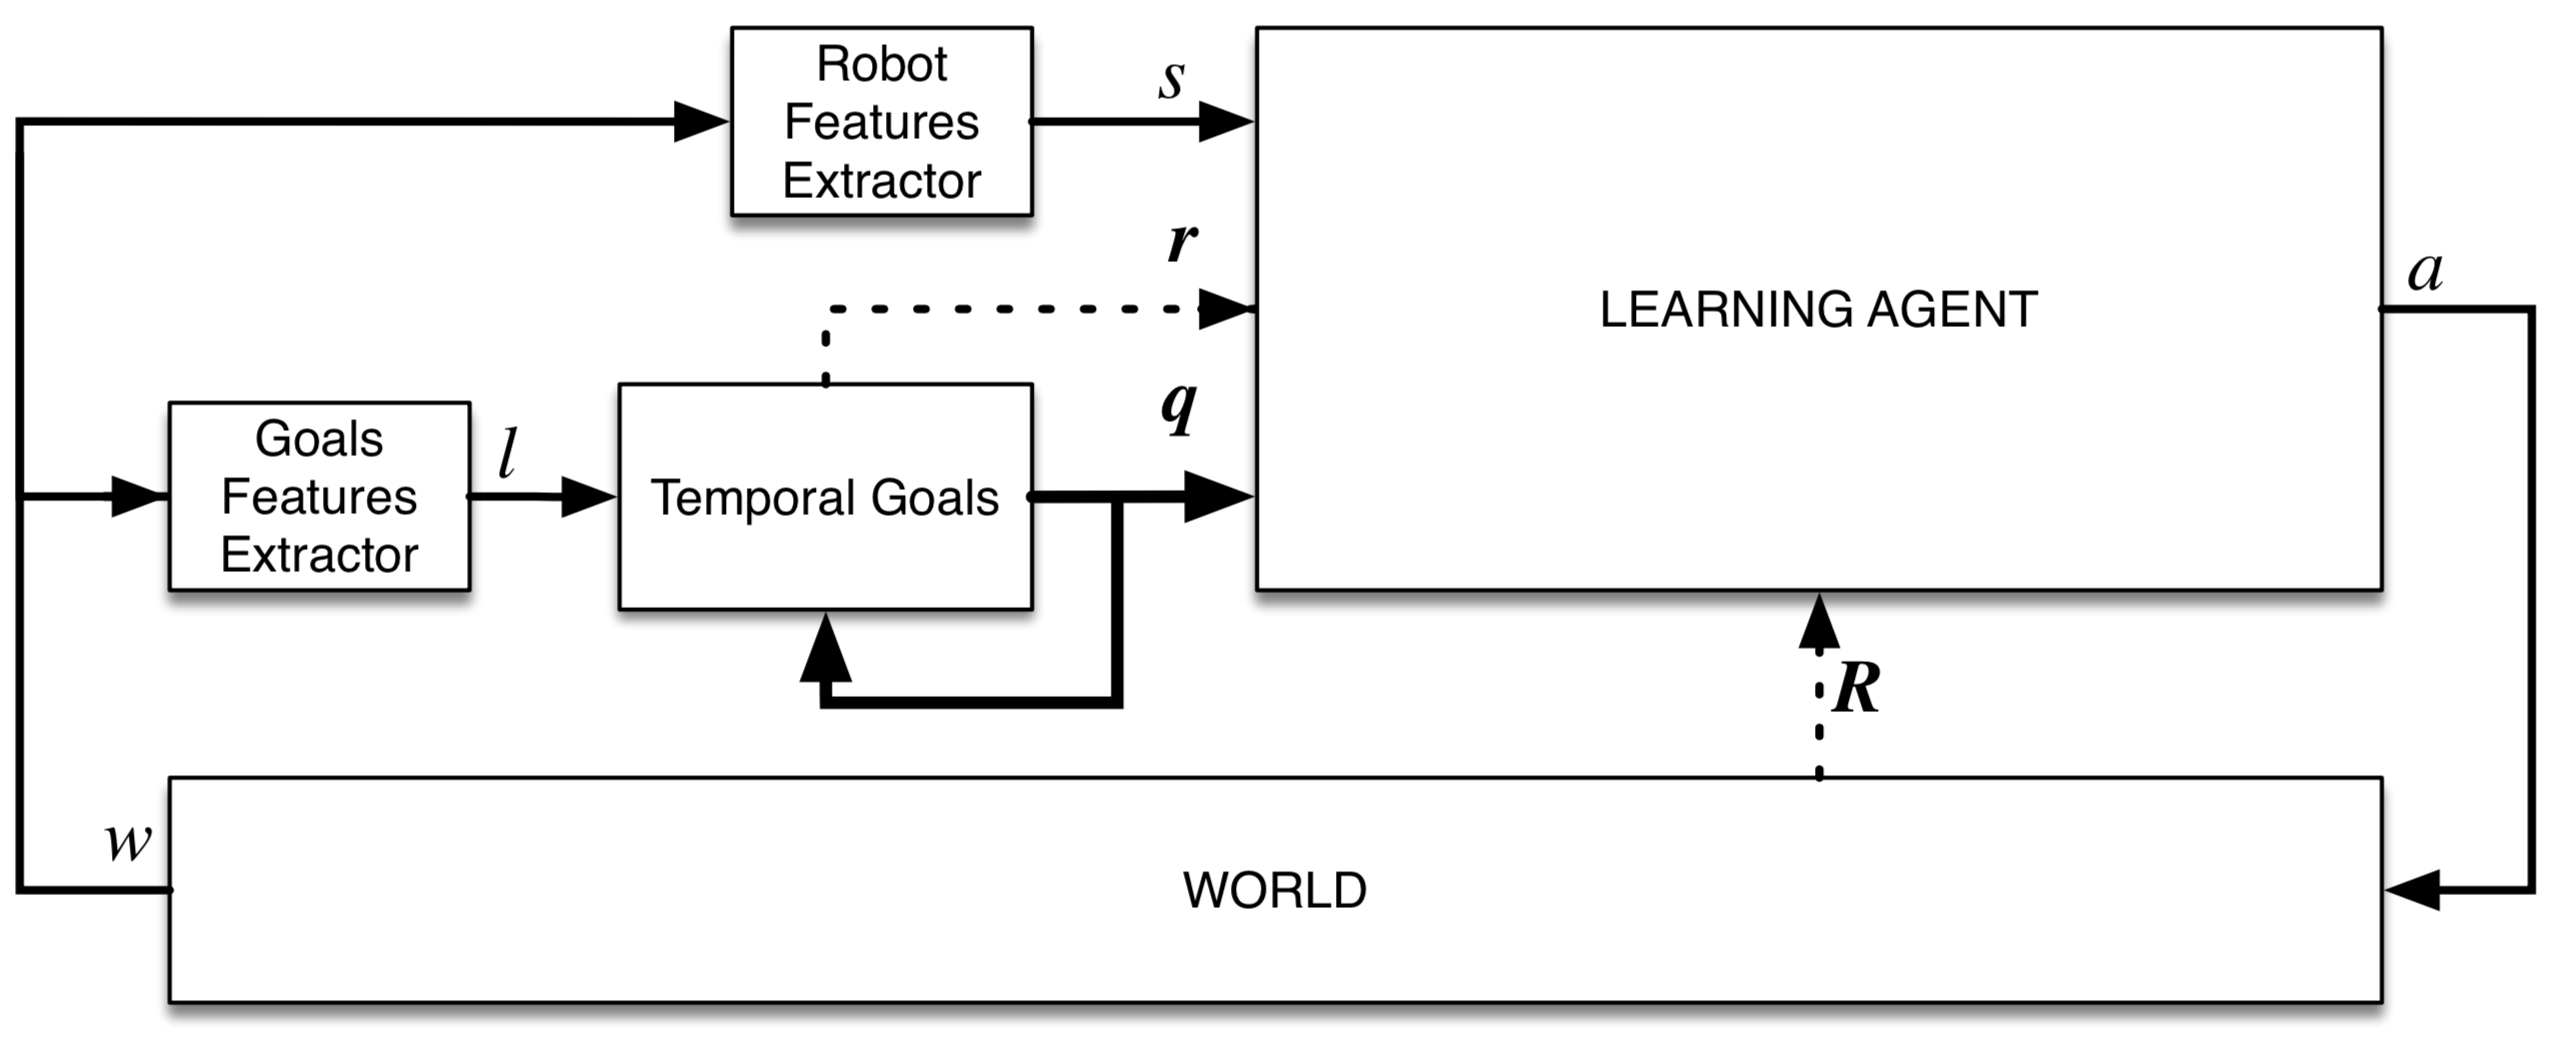
\includegraphics[width=0.85\textwidth]{images/rl-temporalgoals-pipeline.png}
    \caption{TODO: description.}
    \label{fig:rl-temporalgoals-pipeline}
\end{figure}

\subsection{Examples}
How it can be used to train a RL model.
